\section{Thursday, November 17th}
\subsection{Z Transform (Continued)}
Today we will continue our journey through the Z Transform.

Last time we ended with the Time-Shift Property:
\begin{align*}
    x(n) &\zt \Xhat
    \\
    x(n-N) &\zt \zN\Xhat
\end{align*}

If $N>0$, then the RHS of the 2nd line can be written as $\to\frac\Xhat\zpN$.
\begin{important}
Q: What could potentially go wrong?
\end{important}
A: You could have a pole at $z=0$, which gets canceled out with the numerator thus leading to the loss of a solution -- note that this depends on what $\Xhat$ is.

If $N<0$, then we could potentially lose $\infty$ from the RoC.\\
Example $N=-1$: $u(n+1)\zt\frac{z^2}{z-1},\quad1<|z|<\infty$ where we exclude $z=\infty$ as we diverge there.

\hrulefill

\subsection{Time-Reversal Property}
Given $x(n)\zt\Xhat=\displaystyle\sum_n x(z)\zn$, let us define the time reversed $x$ as $x_{\text{TR}}(n)\triangleq x(-n)$. \\
Find the Z Transform of $x_{\text{TR}}(n)$.
\begin{align*}
    \Xshat{TR} 
    &= \sum_n x(-n)\zn
    \\
    &= \sum_\ell x(\ell)\zpl
    &&\text{[Change of Variables: $\ell=-n$]}
    \\
    &= \sum_\ell x(\ell)(\zinv)^{-\ell}
    \\
    &=\Xphat{\zinv}
\end{align*}

Let us say that the ROC for $x$ is $R_x=\{z\in\mathbb C\ \Big|\ r_1<|z|<r_2\}$.

Then $R_{x_{\text{TR}}} = \{z\in\mathbb C\ \Big|\ r_1<|z^{-1}|<r_2\}
= \{z\in\mathbb C\ \Big|\ \frac1{r_1}<|z|<\frac1{r_2}\}$.

Graphically we can see that the pole-zero plots of $x(n)$ as well as that of $x_{\text{TR}}(n)$ are both two-sided.

\subsection{Multiplication by a complex expon.}
Given $x(n)\zt\Xhat=\displaystyle\sum_n x(z)\zn$, let us define the signal $q(n)\triangleq\zopn x(n)$. \\
Find the Z Transform and RoC of this signal.
\begin{align*}
    \hat Q(z) 
    &= \sum_n \zopn x(n)\zn
    \\
    &= \sum_n x(n)\left(\frac{z}{z_0}\right)^{-n}
    \\
    &= \Xphat{\frac{z}{z_0}}
\end{align*}
where $z_0=r_0e^{i\omega_0}$.

Since $R_x=\{z\in\mathbb C\ \Big|\ r_1<|z|<r_2\}$,

we have $R_{q} = \{z\in\mathbb C\ \Big|\ r_1<\left|\frac{z}{z_0}\right|<r_2\}
= \{z\in\mathbb C\ \Big|\ r_1<\frac{|z|}{r_0}<r_2\}
= \{z\in\mathbb C\ \Big|\ {r_0}r_1<{|z|}<{r_0}r_2\}$.

Note that if $|z_0|>1$ then you will have an \textbf{expansion} between the two circles that the RoC sits.

Note that if $|z_0|<1$ then you will have a \textbf{contraction} between the two circles that the RoC sits.

\subsection{Suddenly-Applied Sinusoidal Excitation}
Find the Z Transform of $r(n)=\cos(\omega_0 n) u(n)$.

We can start by actually simplifying: $r(n)=\cos(\omega_0 n) u(n) = \frac12e^{i\omega_0 n}u(n)+\frac12e^{-i\omega_0 n}u(n)$.

If we let $z_0=e^{i\omega_0}$, we can use the fact that $u(n)\zt \hat U(z)=\frac{z}{z-1},\quad1<|z|$\\
as well as the fact that $q(n)=\zopn x(n)\zt \hat Q(z)=\Xphat{\frac{z}{z_0}}$,\\
we can then realize $z_0^n u(n)
=e^{i\omega_0n}u(n)
\zt
\hat U\left({\frac{z}{z_0}}\right)
=\hat U\left({\frac{z}{e^{i\omega_0}}}\right)
=\frac{\frac{z}{e^{i\omega_0}}}{\frac{z}{e^{i\omega_0}}-1}
=\frac{{e^{-i\omega_0}{z}}}{{e^{-i\omega_0}{z}}-1}$.\\
Likewise, $z_0^{-n} u(n)
=e^{-i\omega_0n}u(n)
\zt
\hat U\left({\frac{z}{e^{-i\omega_0}}}\right)
=\frac{{e^{i\omega_0}{z}}}{{e^{i\omega_0}{z}}-1}$
\begin{align*}
    \hat R(z) 
    &=
    \frac12
    \left[
        \frac{{e^{-i\omega_0}{z}}}{{e^{-i\omega_0}{z}}-1}
        +
        \frac{{e^{i\omega_0}{z}}}{{e^{i\omega_0}{z}}-1}
    \right]
    \\
    &=
    \frac12
    \left[
        \frac{{{z}}}{{{z}}-e^{i\omega_0}}
        +
        \frac{{{z}}}{{{z}}-e^{-i\omega_0}}
    \right]
    &&\text{[Multiply by $\pm\frac{e^{i\omega_0}}{e^{i\omega_0}}$]}
    \\
    &=
    \frac{z}2
    \left[
        \frac{1}{{{z}}-e^{i\omega_0}}
        +
        \frac{1}{{{z}}-e^{-i\omega_0}}
    \right]
    &&\text{[Pull the $z$ out]}
    \\
    &=
    \frac{z}2
    \left[
        \frac{z-e^{-i\omega_0} + z-e^{i\omega_0}}{(z-e^{i\omega_0})(z-e^{-i\omega_0})}
    \right]
    &&\text{[Common Denominator]}
    \\
    \hat R(z) 
    &=
    \frac{z(z-\cos(\omega_0))}{(z-e^{i\omega_0})(z-e^{-i\omega_0})}
    &&\left[\cos(\omega_0)=\frac{e^{i\omega_0}+e^{-i\omega_0}}{2}\right]
\end{align*}
The Pole-Zero diagram will have zeros at $z=0, \cos(\omega_0)$ and poles on the unit circle at $z=e^{i\omega_0}, e^{-i\omega_0}$, one rotated by an angle of $+\omega_0$ and the other rotated by $-\omega_0$.\\
Note that this statement assumes that $\omega_0$ is positive.

Because this system is causal, the RoC will extend outwards form the unit circle.

\begin{shaded}
Note that if $z=\xi_0$ is a zero of the original function, now $\frac{z}{e^{i\omega_0}}=\xi_0$ is a zero of $z=\xi_0e^{i\omega_0}$.
\end{shaded}

\subsection{Uniqueness of the Z Transform}
If you are told that the Z Transform is rational then it is unique up to a constant factor, $H_0$:
\begin{equation}\label{eq:ratzt}
    \hat H(z) 
    = H_0 \frac{\displaystyle\prod_{x_i\in Z} (z-x_i)}{\displaystyle\prod_{p\in P} (z-p)}
\end{equation}
where $Z$ is the set of zeros and $P$ is the set of poles. 

In the homework, you shall work with this much more. If I tell you that the DC Gain of a Filter is $1$, you know that the transfer function $\hat H(z)\left.\right|_{z=1}=1$ as $e^{i0}=1\zt z=1$. Then you can solve for the constant $H_0$ by setting \eqref{eq:ratzt}, evaluated at the DC Gain, to 1.

\subsection{DT-LTI System Example Questions}
Consider a DT-LTI filter ${H}$ that is causal and has a rational $\hat H(z)$, with\\ 
$x(n)=1 \to \boxed{H} \to y(n)=-\frac{4}{3}$. 

The pole-zero diagram has poles at $z=-\frac{1}{2}, \frac{3}{4}$, and a zero at $z=\frac{3}{2}$. 
\begin{shaded}
Questions:
\begin{enumerate}
    \item Warmup: Is H BIBO stable?
    \item What is $\hat{H}(z)$ (and then find $h(n)$ from it).
\end{enumerate}
\end{shaded}
Answers:
\begin{enumerate}
    \item First let us find the RoC. Since $H$ is causal (or right-sided), we know that the RoC extends outwards from the outer most pole.
    This leads to $R_h=\{z\in\mathbb C\Big|\frac34<|z|\}$.
    Therefore we know $H$ is BIBO stable as the unit circle is included in the RoC.
    \item $\hat{H}(z)=A\frac{z-\frac32}{(z+\frac12)(z-\frac34)},\quad\frac34<|z|$ where $A$ is some scaling factor.
\end{enumerate}

\subsubsection{Finding the Unique Z Transform}
We can find $A$ using the fact that $x(n)=1=\zopn\to\boxed{H}\to y(n)=-\frac43$ is analogous to:\\
$x(n)=\zopn\to\boxed{\Hhat}\to y(n)=\Hphat{z_0}\zopn$.

$x(n)=1=z_0^n$ for $z_0=1$, therefore $\hat{H}(1)=-\frac{4}{3}$. 
\begin{align*}
    \hat{H}(z)
    &=A\frac{z-\frac32}{(z+\frac12)(z-\frac34)}
    &&\text{[Original Z Transform]}
    \\
    \hat{H}(1)
    &=A\frac{1-\frac32}{(1+\frac12)(1-\frac34)} = -\frac43
    &&\text{[Plug in $z=1$ to use the known value of $\hat{H}(1)$]}
    \\
    -\frac43
    &=
    A\frac{1-\frac32}{(1+\frac12)(1-\frac34)} = -\frac{4A}3
    \\
    \frac{4A}3 &= \frac43
    \implies
    \boxed{A = 1}
\end{align*}

\subsubsection{Finding the Impulse Response}
Let us simplify the task of finding $h(n)$, let us start by finding $h(0)$.

Here's a hint to do so:
\begin{flalign*}
    \Hhat 
    &=\sum_{n=0}^\infty h(n) z^{-n}
    &&\text{[Definition of Z Transform for Causal System]}
    \\
    \Hhat 
    &= h(0) + h(1) \zinv + h(2)\ze{2} + \cdots
    \\
    \implies
    \lim_{z\to\infty}\Hhat 
    &= h(0)
    &&\text{[Zero out all the terms after $h(0)$]}
    \\
    \lim_{z\to\infty}\Hhat 
    &= 0
    &&[\text{order}(\text{denom}\{\hat H\})>\text{order}(\text{numer}\{\hat H\})]
\end{flalign*}
as $\text{order}(\text{denominator}\{\Hhat\})=2,\ \text{order}(\text{numerator}\{\Hhat\})=1$ and $2>1$.

\subsection{Initial Value Theorem}
\begin{shaded}
If a signal or function $h$ is causal -- if $h(n)=0, n<0$ -- then we can find the initial value as such: $\displaystyle\lim_{z\to\infty}\Hhat=h(0)$.
\end{shaded}
Note that casual is a term for systems so we are currently abusing terminology -- we simply mean that the signal is $0$ on the left-side of the origin.

\subsection{Impulse Response from a Z Transform}
To find $h(n)$, we will need to revisit our Calculus days to utilize Partial Fraction Decomposition:
\begin{align*}
    \hat{H}(z)
    =\frac{z-3 / 2}{(z+1 / 2)(z-3 / 4)}
    &=\frac{\alpha}{z+1 / 2}+\frac{\beta}{z-3 / 4}
    \\
    =\frac{z-3 / 2}{(z+1 / 2)(z-3 / 4)}
    &=\frac{(\alpha+\beta)z+(\frac\beta2-\frac{3\alpha}{4})}{(z+1 / 2)(z-3 / 4)}
    &&\text{[Common Denominator]}
    \\
    &\implies
    \alpha+\beta=1,\ \frac\beta2-\frac{3\alpha}{4}=-\frac32
    &&\text{[Pattern-match like-terms]}
    \\
    &\implies
    \alpha=\frac85, \ \beta=-\frac35
    &&\text{[Solve the system]}
\end{align*}

Therefore,
\begin{align*}
    \hat{H}(z)
    &=\frac{8}{5} \frac{1}{z+\frac{1}{2}}
    &&-\frac{3}{5} \frac{1}{z-\frac{3}{4}}
    &&&\text{[PFD form with respective $\alpha,\beta$]}
    \\
    &=\frac{8}{5}\zinv\left(\frac{z}{z-\frac{-1}{2}}\right) 
    &&-\frac{3}{5}\zinv\left(\frac{z}{z-\frac{3}{4}}\right)
    \\
    h(n)
    &=\frac{8}{5}\zinv\left(-\frac{1}{2}\right)^{n} u(n)
    &&-\frac{3}{5}\zinv\left(\frac{3}{4}\right)^{n} u(n)
    &&&[\dagger: \lambda_1=-\frac12, \lambda_2=\frac34]
    \\
    h(n)
    &=\frac{8}{5}\left(-\frac{1}{2}\right)^{n-1} u(n-1)
    &&-\frac{3}{5}\left(\frac{3}{4}\right)^{n-1} u(n-1)
    &&&\text{[Delay by one sample]}
\end{align*}
$^\dagger$ as $\lambda^n u(n)\zt \frac1{1-\lambda\zinv}=\frac{z}{z-\lambda},\quad|\lambda|<|z|$.

Sanity Check: $h(0)=0$ is satisfied -- due to the unit step functions!

\subsection{Differentiation in \texorpdfstring{$z$}{z}}
Given $x(n)\zt \Xhat$, show that $nx(n)\zt -z\dv{\Xhat}{z}$.
\begin{align*}
    \Xhat 
    &= \sum_n x(n)\zn
    \\
    \dv{\Xhat}{z} 
    &= -\sum_n n x(n) \ze{n-1}
    &&\text{[Differentiate both sides]}
    \\
    -z\dv{\Xhat}{z} 
    &= \underbrace{\sum_n \underbrace{n x(n)} \zn}_{\mathcal Z\{nx(n)\}}
    &&\text{[Multiply both sides by $-z$]}
\end{align*}

\subsection{ Impulse Response from Z Transforms with Differentiation}
Given $\hat Q(z)=\frac z{(z-1)^2}$, what is $q(n)$?

We know that $u(n)\zt \underbrace{\frac{z}{z-1}}_{\hat U(z)}$ which can take the derivative of:
\begin{align*}
    \dv{\hat U(z)}{z} &= \frac{\cancel{z}-1\cancel{-z}}{(z-1)^2}=\frac{-1}{(z-1)^2}
    &&\text{[Differentiate $\mathcal Z\{u(n)\}$ wrt $z$]}
    \\
    -z\dv{\hat U(z)}{z} &= \frac{z}{(z-1)^2} = \hat Q(z)
    &&\text{[Multiply both sides by $-z$]}
\end{align*}

Therefore using the differentiation property we just proved above, $q(n)=n u(n)$.

If we were to look at the dotplot of this, we would see a discrete ReLU: $0\ (\forall n\le0)$ and $n\ (\forall n\in\mathbb Z^+)$.

\subsection{ DT-LTI Systems Described by LCCDEs}
\begin{align*}
    a_0 y(n) + a_1 y(n-1) + \cdots + a_N y(n-N)
    &=
    b_0 x(n) + b_1 x(n-1) + \cdots + b_M x(n-M)
    \\
    \sum_{k=0}^N a_k y(n-k)
    &= \sum_{m=0}^M b_m x(n-m)
    \\
    \text{Take the Z Transform of both sides}&\text{, use the Time-Shift Property:}
    \\
    \sum_{k=0}^N a_k \hat Y(z) z^{-k}
    &= \sum_{m=0}^M b_m \hat X(z) z^{-m}
    \\
    \left[\sum_{k=0}^N a_k z^{-k}\right] \hat Y(z)
    &= 
    \left[\sum_{m=0}^M b_m z^{-m}\right] \hat X(z)
    \\
    \left[\sum_{k=0}^N a_k z^{-k}\right] \frac{\hat Y(z)}{\hat X(z)}
    &= 
    \left[\sum_{m=0}^M b_m z^{-m}\right]
    \\
    \hat H(z)
    &=\hat Y(z)/\hat X(z)
    \\
    \hat H(z)
    &= 
    \frac{\sum_{m=0}^M b_m z^{-m}}
         {\sum_{k=0}^N a_k z^{-k}}
    \\
    &= 
    \frac{b_0 + b_1 z^{-1} + \cdots + b_M \ze{M}}
         {a_0 + a_1 z^{-1} + \cdots + a_N \ze{N}}
\end{align*}
\begin{shaded}
Big Idea: Any DT-LTI Systems Describable by an LCCDE has a rational transfer function.
\end{shaded}

\subsection{ Feedback Stabilization}
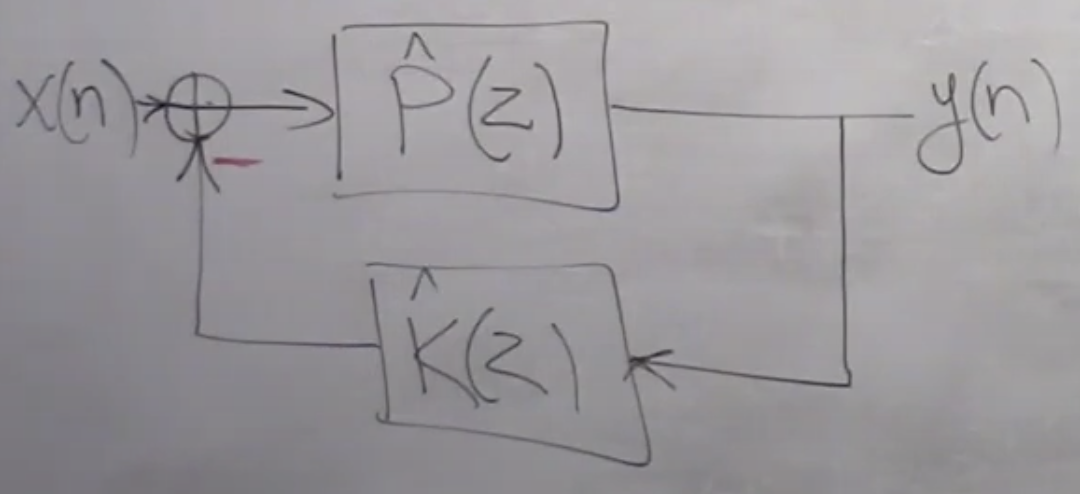
\includegraphics[scale=0.2]{lectures/wk12/img/system.png}
$\implies$
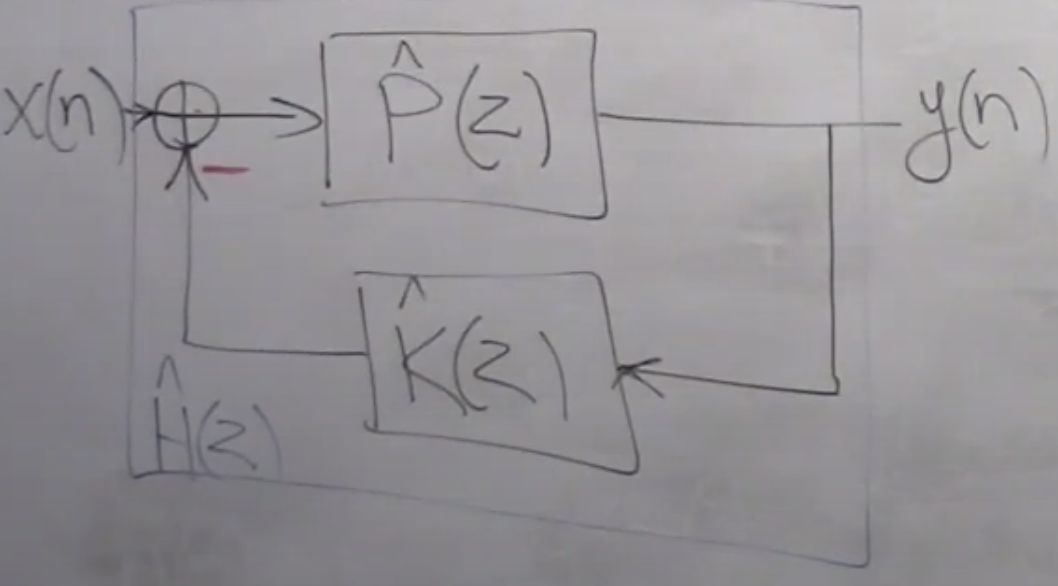
\includegraphics[scale=0.17]{lectures/wk12/img/system2.png}

Reformulating the left system as the right, we can say that $\Hhat=\frac{\hat P(z)}{1+\hat K(z)\hat P(z)}$.

\[
    p(n)=2^n u(n)
\]
is exponential growth so not only is not BIBO stable, but it also does not have a DTFT -- it is faster than polynomial growth.

\begin{align*}
    \hat P(z) 
    &=
    \frac1{1-2\zinv}=\frac{z}{z-2},\ 2<|z|
    &&\text{as }\lambda^n u(n)\zt \frac1{1-\lambda\zinv}=\frac{z}{z-\lambda},\quad|\lambda|<|z|
\end{align*}

\subsection{ Shift Register with Gain Factors}
\[
    k(n) = \alpha\delta(n-1)
\]
can be seen as a Shift Register with Gain Factor = $\alpha$.

This signal has the following Z Transform:
\begin{align*}
    \hat K(z) 
    &= \alpha \mathcal Z\{\delta(n-1)\}
    &&\delta(n) \zt \sum_n \delta(n)\zn=1
    \\
    \implies
    \hat K(z) 
    &= \alpha \zinv
    &&\delta(n-1) \zt \sum_n \delta(n-1)\zn=\zinv
    \\
    \implies
    \hat H(z) 
    &= \frac{z}{z-(2-\alpha)}
    \\
    &= \frac{1}{1-(2-\alpha)\zinv}
    \\
    \implies
    h(n)
    &=
    (2-\alpha)^n u(n),\ |2-\alpha|<1.
\end{align*}
with a zero at the origin and a pole at $z=2-\alpha$.

We want $-1<2-\alpha<1$ which is the same as saying $1<\alpha \cap \alpha<3$ or $\boxed{1<\alpha<3}.\hfill\square$

